\chapter{Imagerie fonctionnelle sous stimulation vestibulaire}\label{chapIII}

% VolkerComment
% You have to extent significantly the first paragraph and link it to the previous chapter. For the following subsections you have to seperated Geoffrey's development from your developments. When you started your PhD the one-photon system was already developed by Geoffrey. You have to review this development in all details to prepare the chapter where you present the two-photon RLS and your developments. Especially, you have to talk about the fiber delivery of the laser onto the rotating platform. Do not mix this presentation with any developments that yo did later for the 2PRLS. Your contribution comes when you talk about the challenges posed by treating the recorded large data sets and the necessity of the development of an analysis pipeline. Introduce well the analysis challenges and the requirement that a good analysis pipeline should fulfill. Then you write an entire chapter to detail your easyRLS development. This routine became the bases for the data analysis in the paper and is our work horse in the group until today. This development gave you a first publication.


% TODO Papier Current Biology

%%%%%%%%%%%%%%%%%%%%%%%%%%%%%%%%%%%
%%%%%%%%%%%%%%%%%%%%%%%%%%%%%%%%%%%
%%%%%%%%%%%%%%%%%%%%%%%%%%%%%%%%%%%
\section{Microscope rotatif}

% transition
Dans le chapitre précédent, je montre comment tester le comportement d'intégration visuo-vestibulaire dans un environnement en réalité virtuelle. L'objectif est d'observer l'activité du cerveau lors d'un tel comportement. Pour cela, il faut un système capable de réaliser l'enregistrement neuronal en même temps que la stimulation des systèmes vestibulaire et visuel. Cet objectif présente plusieurs difficultés : exciter le système vestibulaire tout en gardant le poisson fixe par rapport à l'objectif de microscope et contrôler son environnement visuel en dépit du laser d'excitation de fluorescence. Dans ce chapitre, je m'intéresse à la partie vestibulaire.

Pour stimuler le système vestibulaire tout en gardant le poisson fixe par rapport à l'objectif, une option est d'agir directement sur l'organe vestibulaire sans bouger la larve. C'est la solution adoptée par Favre Bulle \emph{et al} dans un article publié en 2017 \cite{favre-bulle_optical_2017}. Les auteurs ont utilisé des pinces optiques pour stimuler directement les otolithes. Cette solution est limitée car il n'est pas possible de calibrer la force appliquée, la concentration du laser produit un échauffement qui limite la durée maximale de la stimulation, et la gamme de force applicable est restreinte.

Au Laboratoire Jean Perrin, Geoffrey Migault et Volker Bormuth se sont tourné vers une autre option : tourner réellement le poisson pour que la gravité bouge ses otolithes.
% Papi Jean est mort. Je m'arrête un moment.
Cette deuxième solution est plus performante, car elle reproduit réellement la stimulation vestibulaire sans les limitations dues au pinces optiques, mais elle nécessite des développements techniques avancés pour être appliquée sous microscope. En effet, pour conserver le microscope fixe par rapport à un poisson mobile, il faut construire un microscope rotatif, tout en gardant les conditions de stabilité nécessaires à l'imagerie. Un microscope à feuille de lumière rotatif capable de mesurer l'activité du cerveau pendant une stimulation vestibulaire réelle a donc été développé \cite{migault_whole-brain_2018}.

\subsection{Description du montage}

\subsubsection{Unité d'illumination}

Un microscope à feuille de lumière par balayage est généralement constitué de deux bras optiques formant un téléscope de manière à placer le miroir rotatif galvanométrique de balayage dans le plan congugé de l'échantillon. Ainsi, son mouvement de rotation est transformé en une pure translation du faisceau au niveau de l'échantillon. Ce montage est volumineux et inadapté à un microscope rotatif. Il a donc fallu le miniaturiser et garantir sa stabilité. Les téléscopes ont été remplacés par des objectifs de microscope. Le plan de Fourier n'étant pas accessible à cause de la distance frontale arrière, le miroir galvanométrique est légèrement hors du plan conjugué, ce qui introduit une rotation du faisceau dans l'échantillon en plus de la translation. Cette rotation reste cependant faible (<0.4°), et compatible avec une feuille de lumière par balayage.  
L'unité d'illumination est composée d'un connecteur de fibre monté sur un positionneur piézoélectrique et de deux objectifs en montage confocal de part et d'autre d'un miroir galvanométrique. 

\begin{figure}
\centering
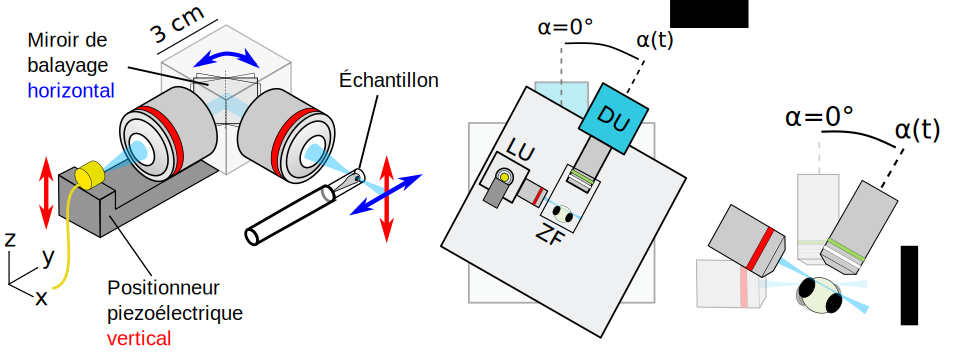
\includegraphics[width=0.8\textwidth]{./files/miniature_light-sheet.svg.png}
\caption{Schéma extrait de l'article \cite{migault_whole-brain_2018}. Le module miniature peut être monté sur un microscope rotatif.
}
\end{figure}

\subsubsection{Unité de détection}

L'enjeu pour une unité de détection rapide est de permettre l'enregistrement avec une durée d'exposition la plus courte possible tout en maintenant un rapport signal à bruit suffisant. Pour collecter beaucoup de lumière, il faut une grande ouverture numérique, et donc une distance de travail faible. Cependant, pour une imagerie à champ large, il faut un grandissement faible. La solution retenue est un objectif Olympus d'ouverture numérique 1 et de grandissement x20. Le grandissement est donné pour une lentille de tube de 180 mm, mais une lentille de tube de 150 mm a été utilisée, ce qui donne donc un grandissement de x16.667. Un pixel de la caméra mesure 6.5 µm, ce qui donne un pixel objet de 0.39 µm. Le capteur CMOS est un carré de 2048 pixels de côté, ce qui donne un champ objet de 0.8 mm. Le champ objet correspond à la longueur du cerveau, mais le pixel objet est très petit par rapport à un neurone. Pour limiter la quantité de données à enregistrer et augmenter le rapport signal à bruit, on peut combiner par les pixels de la caméra, opération appellée \emph{binning}. Cela donne un pixel objet de 0.78 µm.

\begin{figure}
\centering
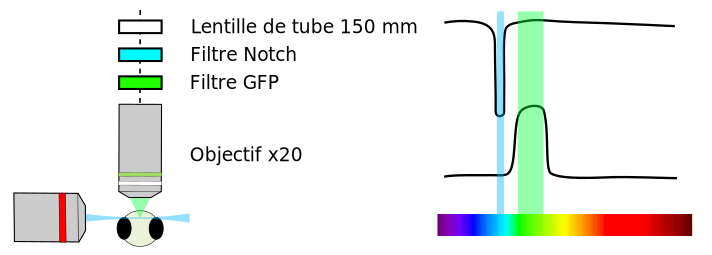
\includegraphics[width=0.8\textwidth]{./files/detection_unit.svg.png}
\caption{Schéma du filtrage spectral dans le bras de détection. Le filtre notch (\emph{encoche}) est très étroit et rejette la longueur d'onde du laser (488 nm). Le filtre GFP et plus large et transmet seulement une bande autour de la fréquence de la GFP (525 nm).}
% 1e-5 à 488 nm pour GFP
% 1e-6 à 488 nm pour Notch
\end{figure}

% VolkerComment
% Originally, we did the experiments only with the notch filter. All photons emitted by the fluorophore were then collected which maximizes the signal. The GFP filter helps to block some additionally excited autofluorescence in the tissue. With the GFP filter the notch filter is not really anymore necessary. You can keep your figure but show the real GFP filter transmission spectrum in this case !


Pour obtenir un bon rapport signal à bruit, il faut réduire la lumière parasite. Une source puissante est le laser d'illumination, elle peut être bloquée spécifiquement avec un filtre coup bande très étroit à sa longueur d'onde. Un filtre GFP (passe-bande à la longueur d'onde de la GFP) permet de filtrer davantage l'autofluorescence des tissus. Après ce filtrage, les bruits restants sont le bruit de photon et le bruit numérique. Le bruit numérique pourrait être réduit avec un système de refroidissement prévu sur la caméra, mais celui-ci est trop encombrant pour le microscope rotatif, et a donc été retiré. Le bruit de photon ne peut être réduit qu'avec des meilleures sondes calciques ou en exposant plus longtemps, mais il est négligeable devant le bruit numérique d'une caméra non refroidie. Le bruit numérique présente une structure liée à la constitution interne du capteur et qui fait apparaître des raies de pixel et la ligne médiale de l'obturateur déroulant.

% VolkerComment
% No! We do not filter out light from light sources in the room! The systems are shielded such that this light does not enter the detection path . The GFP filter filters additional excited autofluorescence.

% L'unité de détection est composée d'un objectif à immersion (le poisson est dans l'eau) monté sur un positionneur piézoélectrique, d'une lentille de tube, d'un filtre coupe-bande, d'un filtre GFP, et d'une caméra.

\subsubsection{Stabilité mécanique}

Le tout pèse environ 2 kg (?) et tient sur une plaque de 50 cm de côté fixée à un moteur à grand couple et grande précision. Le moteur dispose d'un grand rotor permettant une large zone de fixation qui minimise les déformations mécaniques de la plaque qui soutient le microscope. Nous avons caractérisé précisément l'instabilité liée à la rotation du microscope à l'aide de billes micrométriques fluorescentes.

\begin{figure}
\centering
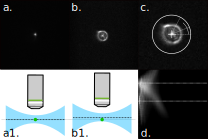
\includegraphics[width=0.8\textwidth]{./files/bead_position.svg.png}
\caption{Schéma des étapes pour estimer avec précision la position d'une bille fluorescente.\\
a. Image d'une bille dans le plan focal de l'objectif (a1)\\
b. Image d'une bille hors du plan focal de l'objectif (a2)\\
c. Établissement du profil radial par moyennage autour du centre de gravité de l'image\\
d. Profil cylindrique de la figure de diffraction constitué du profil radial pour plusieurs positions de l'objectif espacées de 20 nm. Les traits pointillés correspondent aux plans (a) et (b). La corrélation verticale du profil cylindrique pour plusieurs positions du microscope donne avec précision le déplacement de la bille.}
\end{figure}

Une bille fluorescente de 1 µm est éclairée transversalement par le laser d'excitation, qui coincide avec le plan focal de l'objectif de détection. Elle est imagée pour plusieurs positions hors focus de l'objectif, ce qui fait apparaître des franges d'interférence. Un profil cylindrique de ces franges est réalisé pour plusieurs positions du microscope et à plusieurs intervalles de temps ce qui permet de mettre en évidence le déplacement latéral et vertical de la bille au cours du temps et en fonction de la position du microscope. Cette technique a l'avantage d'être précise (de l'ordre de 100 nm) et robuste aux variations liées au photoblanchiment. Elle a permis de montrer que lors de la rotation du microscope, le déplacement reste inférieur à 500 nm dans la direction verticale et 2 µm dans la direction latérale (cette dernière peut être corrigée lors de l'analyse comme on le voit plus tard).

\subsection{Nappe laser par balayage}

\subsubsection{Ouverture numérique optimale}

Le volume d'un cerveau de larve de poisson zèbre mesure 400 µm de largeur × 800 µm de longueur × 300 µm de hauteur et est situé sur le dessus de la larve. Afin de minimiser l'épaisseur de tissus traversée, on place donc l'objectif de détection sur la partie supérieure. Le laser peut donc être placé sur le côté. Les yeux sont très pigmentés et la lumière ne passe pas à travers, ce qui crée une zone d'ombre entre les yeux. Certains laboratoires qui sont intéressés par ces régions appartenant au télencéphale et au diencéphale peuvent donc ajouter un deuxième laser à l'avant pour éclairer cette région.

Pour produire un faisceau laser le plus fin possible sur une longueur de 400 µm, il faut minimiser la largeur après 200 µm de propagation avec comme variable le waist $w_0$ placé au milieu de l'échantillon :

$$
w(z) = w_0 \, \sqrt{ 1+ {\left( \frac{z}{z_\mathrm{R}} \right)}^2 } \qquad z_\mathrm{R} = \frac{n \pi w_0^2 }{\lambda}
$$

\begin{figure}
\centering
\includegraphics[width=0.8\textwidth]{./files/possible-waist_1P.png}
\caption{On voit ici la demi largeur du profil gaussien à 488 nm dans l'eau pour différentes valeurs du waist. Le trait en pointillé montre le rayon d'un neurone. On cherche à minimiser l'épaisseur du faisceau entre -100 µm à 100 µm. Le trait épais marque la position optimale pour ce critère (les autres profils sont tous plus larges à 100 µm du centre). L'ouverture numérique associée vaut $ \mathrm{NA} = n\sin(\lambda/\pi n w_0) $.}
\end{figure}

% VolkerComment
% Indicate the NA used for the different curves.

Un waist trop petit est trop divergeant, et donc trop large sur les bords, mais un waist trop large limite la résolution. Il faut donc donc trouver un optimum. La taille d'un neurone étant de 8 µm environ, des valeurs inférieures sont souhaitables.

Une valeur de waist possible pour un échantillon de 400 µm est de 3 µm à 488 nm et de 5 µm à 915 nm. Pour ces valeurs, la largeur du faisceau à 488 nm vaut 3 µm au centre et 10 µm sur les bords du cerveau. À 915 nm c'est 5 µm au centre et 14 µm sur les bords mais il faut aussi prendre en compte l'effet deux photons. En pratique, la plupart des neurones sont situés entre -150 µm et +150 µm, la largeur du faisceau aux extrémités n'est donc pas critique.

\subsubsection{Balayage horizontal et vertical}

Pour effectuer le balayage, on déplace le faisceau horizontalement. Pour que l'intensité soit homogène sur une image, il faut adopter une vitesse de déplacement constante. Il est alors possible de faire un aller simple ou des allers-retours en nombre entier pendant le temps d'exposition. Pour obtenir une image volumétrique, il suffit de répéter l'opération pour plusieurs couches, en changeant le plan focal de l'objectif de détection et la position vertical de la nappe. Procéder de cette manière couche après couche force à attendre entre deux couches pour laisser le temps aux éléments mécaniques de se positionner, ce qui prend un temps (environ 10 ms) non négligeable pour des durées d'exposition courtes. Il est également possible de bouger les éléments mécaniques de manière continue en balayant en aller simple. Les couches sont donc légèrement obliques, mais on gagne considérablement en fréquence d'acquisition. Cela est possible grâce au mode "synchronous readout" de la caméra qui permet de lire les valeurs d'une ligne de pixels tout en exposant une autre.


\begin{figure}
\centering
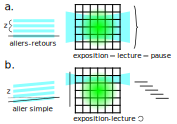
\includegraphics[width=0.6\textwidth]{./files/schema_balayage.svg.png}
\caption{Différents modes de balayage et de lecture du capteur CMOS. Les couches z sucessives sont représentées à gauche, le capteur (dans le plan xy) est représenté à droite.\\
a. Balayage par allers-retours lors de l'exposition de tous les pixels, puis lecture de tous les pixels et déplacement à la couche suivante. Le déplacement étant lent, une pause est nécessaire. Pas d'exposition pendant la pause\\
b. Balayage par aller simple lors de l'exposition, lecture successives des rangées de pixels et ré-exposition immédiate. Le déplacement vertical est continu à vitesse constante, les couches en z sont légèrement obliques. Le cycle exposition-lecture est décalé dans le temps pour chaque rangée de pixels.}
\end{figure}
% Add a figure that shows the different scan protocols and that explains the camera readout

Pour un temps d'exposition par couche de 10 ms en mode d'acquisition continu, on peut par exemple réaliser un scan du cerveau à 2,5 Hz en 30 couches espacées de 8µm. Cela permet d'imager la majeure partie du cerveau du poisson. Les couches les plus profondes sont moins nettes car le signal traverse plus de tissus avant d'atteindre l'objectif, et la zone située entre les yeux reste dans l'ombre si on n'utilise qu'un laser. Mais chaque neurone visible est imagé à une fréquence de 2.5 Hz.

% \subsubsection{Ordres de grandeur}
% -> Partie microscope





% \subsection{Caractérisation}

%%%%%%%%%%%%%%%%%%%%%%%%%%%%%%%%%%%
%%%%%%%%%%%%%%%%%%%%%%%%%%%%%%%%%%%
%%%%%%%%%%%%%%%%%%%%%%%%%%%%%%%%%%%
\section{Analyse des données}

L'analyse des données produites par le microscope est en enjeu en lui même. En effet, avec des images de 1024$\times$600 pixels, 20 couches et 25 minutes d'enregistrement à 2 volumes par seconde, on obtient 60000 images. Pour des pixels stockés sur 16 bits, cela donne près de 60 Go de données brutes. Dans ce chapitre, je m'intéresse aux stratégies pour traiter ces données. Les chiffres donnés ci-dessus sont ceux utilisés pour les calculs en ordre de grandeur par la suite.

\subsection{Logiciels existants}

\subsubsection{Fiji}

De nombreux laboratoires de biologie réalisent leur analyse d'image avec Fiji (une distribution du logiciel ImageJ). Cet outil générique offre en effet une bonne interface pour visualiser les données tout en y appliquant des transformations élémentaires, mais montre rapidement ses limites en terme de vitesse, d'automatisation, et de robustesse. Les différents laboratoires travaillant en imagerie neuronale se sont donc tournés vers des logiciels spécialisés.

\subsubsection{Suite2P}

Les laboratoires réalisant de l'imagerie deux photons sur le cerveau de rongeur ont des données de petit volume, mais nécessitant des algorithmes sophistiqués avant d'être exploitables. Le logiciel \href{https://www.suite2p.org/}{suite2p} \cite{pachitariu_suite2p_2016}, doté d'une interface graphique intuitive expose une routine puissante pour la correction de mouvement et la détection de cellules par leur activité. Quelques essais sur nos jeux de données ont montré que le logiciel était fonctionnel mais excessivement lent, ce qui rend l'analyse systématique impossible.

\subsubsection{CaImAn}

Plusieurs laboratoires travaillant en microscopie à feuille de lumière analysent leurs données à l'aide de \href{https://github.com/flatironinstitute/CaImAn}{CaImAn} (pour \emph{Calcium Image Analysis}) \cite{giovannucci_caiman_2019}. Ce programme est décliné en deux versions, la version \emph{online} pour l'analyse de données en temps réel sur une expérience en cours, et la version \emph{batch} pour l'analyse de données \emph{a posteriori}. La première nécessite des machines très puissantes pour atteindre le taux d'images par secondes requis alors que la seconde peut être exécutée sur des machines modestes. Le logiciel a été publié en 2019, je l'ai essayé sur nos jeux de données avec des résultats satisfaisants en terme de qualité, quoiqu'un peu lents.

\subsection{Solution utilisée pour l'analyse de nos données}

% VolkerComment
% You have to describe your development of easyRLS a routine in form of a collection of functions that allows in a modular manner to analyze the whole-brain data. Go more in detail.

Aucun logiciel adapté à nos données n'étant disponible à l'époque, nous avons développé nos propres méthodes adaptées à l'imagerie sur plateforme rotative. Les spécifications étant très mouvantes, nous avons adopté une structure modulaire dans laquelle une collection de fonctions peuvent être appliquées optionnellement dans un ordre adapté à chaque jeu de données. Je décris ici les étapes principales de l'analyse, les enjeux techniques, et les pistes d'amélioration.

\subsubsection{Étapes principales de l'analyse de données}

\paragraph{Espace de référence}

Dans la suite de cette section, j'appellerai de manière équivalente (x,y,z,t) les cooordonnées d'un point et les axes dans le repère du poisson. Ces coordonnées sont données dans l'espace de référence RAST (\emph{Right Anterior Superior Time}), c'est-à-dire que l'axe x est orienté vers la droite de la larve, l'axe y vers l'avant, l'axe z vers le haut, et le temps dans le sens naturel.

\begin{figure}
\centering
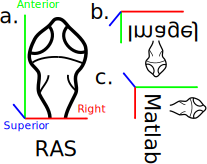
\includegraphics[width=0.6\textwidth]{./files/RAST.svg.png}
\caption{Illustration de la convention d'orientation RAS (a.) et comparaison avec les systèmes de coordonnées naturels de ImageJ (b. coordonnées des pixels d'un écran) et Matlab (c. coordonnées des éléments d'une matrice).}
\end{figure}

% VolkerComment
% Add a figure illustrating the RAST definition and add your wiki page with the corresponding figures about the different coordinate systems used in Matlab, Fiji, cmtk

\paragraph{Alignement temporel}

% VolkerComment
% Start introducing the problem. We have two main problems. Slow thermal drift and fast stimulus induced movements. In addition we have to scope with tissue deformation but normally we discard these runs. Then discuss the different approaches that you developed. Autocorrelation with the first image, autocorrelation with an average image, treatment of all layers independently, estimating the drift per stack based on one layer with good contrast or selecting high contrast landmarks to calculated the drift. Discuss that you developed different approaches: 1. Estimating the fast and slow movements together, 2. Estimating and correcting slow and fast drift sequentially. 3. Correcting the sinusoidal stimulus induced fast component by hand by applying a sinusoidal drift correction with user defined amplitude and phase. Make a figure that illustrates the different approaches

Pour des données à quatre dimensions (x,y,z,t), il est impératif qu'un pixel (x,y,z) représente toujours le même espace objet dans le cerveau. Une première étape consiste donc à aligner toutes les images entre elles. Dans un cas totalement général, le tissus imagé peut connaître des déformations au cours de l'expérience, et il faut estimer et appliquer la transformation inverse. Suite2P et CaImAn fournissent tous les deux des algorithmes de déformation non rigide, mais ces algorithmes sont couteux en temps et il est difficile d'estimer numériquement leur performance. De plus, sur des expériences de vingt minutes, les déformations sont généralement trop faibles pour que cette étape soit réellement nécessaire, nous avons donc opté pour une transformation rigide. Cette transformation rigide peut avoir plusieurs degrés de liberté en translation et rotation. Comme précisé dans la partie sur la conception de la plateforme rotative, nous avons obtenu une excellente stabilité en z, les translations restantes sont donc uniquement selon (x,y), et les rotations sont également négligeables. 

Une difficulté pour trouver cette translation est que l'image peut évoluer le long de l'enregistrement. En effet, la répartition de la concentration de calcium peut significativement fluctuer entre le début et la fin de l'expérience, ce qui dans certains cas empêche tout algorithme naïf de fonctionner. Dans le cas de l'imagerie un photon, le signal d'autofluorescence est suffisant pour qu'une simple autocorrélation sur l'ensemble de l'image permette de trouver le déplacement. Dans le cas de l'imagerie deux photons, ce signal étant bien plus faible, l'autocorrélation sur l'ensemble de l'image est dominée par les changements de fluorescence liée à l'activité de neurones. La solution retenue a donc été de réaliser l'autocorrélation sur une zone de l'image stable pendant toute la durée de l'expérience facilement identifiable à l'œil. C'est par exemple le cas pour un neurone mort qui reste toujours dépolarisé.

Cette étape nécessite donc une supervision rapide à l'œil humain mais fonctionne en général du premier coup et est extrêmement rapide par rapport à tout autre algorithme utilisant l'image entière. De plus, il suffit de réaliser l'opération pour une seule couche et d'extrapoler à tout le volume. Cette étape permet de corriger les déplacements latéraux rapide (x,y) liés directement à la rotation de la plateforme ainsi que la dérive lente en y liée à la contraction du boudin d'agar tenant le poisson.

\paragraph{Alignement sur un cerveau de référence}

Après avoir obtenu une matrice 4D alignée temporellement, il est trivial de réaliser une moyenne temporelle qui permet d'obtenir une image avec un bon rapport signal à bruit et moins dépendante de l'activité des neurones. Ce volume moyenné suivant le temps peut être aligné sur un volume de référence à l'aide de \href{https://www.nitrc.org/projects/cmtk}{CMTK} (\emph{Computational Morphometry Toolkit}). Cela permet d'une part de reporter après analyse les résultats de différents enregistrements sur le même cerveau de référence afin de les comparer et d'autre part d'obtenir un contour du cerveau définissant la région d'intérêt. Cette région d'intérêt peut alternativement être précisée à la main. À partir de ce moment deux voies d'analyse sont possible : par pixel ou par neurone après segmentation.

\paragraph{Analyse de Fourier par pixel}

% VolkerComment
% Add a figure of a typical PSD and show visually how you extract the data
% (PSD = DSP)

Il est intéressant de réaliser certaines analyses directement sur les pixels de l'image. Cela permet d'obtenir des figures avec une bonne résolution et contourne le problème de la segmentation des neurones tout en profitant au mieux de l'échantillonnage permis par la caméra. Cependant, cette approche est coûteuse en calcul car elle opère sur un grand nombre d'éléments. Nous l'avons principalement réservée à l'analyse de Fourier pour une stimulation périodique.
Pour chaque pixel dans la région d'intérêt, on applique la transformée de Fourier discrète sur son profil temporel. Cela donne un pic en amplitude à la fréquence de stimulation et du bruit en dehors. On calcule un rapport signal à bruit comme le rapport de l'amplitude du signal sur l'amplitude du bruit moyennée sur une fenêtre autour du pic de largeur arbitraire. On considère également la phase du pic, qui représente le déphasage dus signal de fluorescence avec le stimulus.
Ces valeurs pour chaque pixels sont ensuite utilisées pour représenter une couleur dans l'espace HSV (\emph{Hue, Saturation, Value} soit Teinte, Saturation, Valeur). La teinte représente le déphasage, la saturation et réglée à 1, et la valeur représente le rapport signal à bruit. 

\paragraph{Segmentation et analyse par neurone}

L'analyse par pixel est pertinante pour des études préliminaires simples car elle est gourmande en calcul, chaque section de neurone (environ 6 µm de diamètre) étant imagée sur environ 40 pixels (pixel objet de 0.8 µm de côté). En regroupant les pixels appartenant au même neurone, on peut réduire le volume de données à traiter tout en conservant leur qualité. Il existe de nombreux algorithmes de segmentation, certains faisant appel aux données temporelles pour tirer profit de l'activité des neurones, d'autre opérant sur l'image moyenne. Nous nous avons pour l'instant uniquement utilisé l'algorithme de ligne de partage des eaux (\emph{watershed}) pour sa simplicité, sa rapidité et ses résultats satisfaisants.

% TODO illustrer pixellation du neurone
% TODO vérifier taille neurone en pixel
% TODO regarder taille de la ROI moyenne par rapport au volume total (somme du masque)

Après segmentation, on définit la valeur d'un neurone comme la moyenne des valeurs des pixels qui le constituent. Chaque segment peut représenter une partie d'un neurone, plusieurs neurones, ou même une zone de l'image sans neurones, mais beaucoup de segments représentent un neurone. Pour environ 200 000 segments, cela réduit l'échantillon à 500 Mo, ce qui permet d'appliquer des algorithmes plus gourmands en ressources en un temps raisonnable.

% TODO vérifier nombre de segments
% TODO baseline, df/f, régression...
% Z-score


% améliorations apportées
% git pour la gestion des versions
% format standard

\subsubsection{Améliorations pratiques et techniques}

\paragraph{Versionnage du code}
Le code utilisé pour l'analyse étant volumineux, sa gestion "génétique" (duplication et mutation) posait problème. J'ai donc mis en place un gestionnaire de version qui a permis d'unir les efforts de développement et de faciliter les mises à jour (correction de bugs, nouvelles fonctionnalités). Son utilisation a eu un effet positif sur la qualité du code, sa réutilisabilité, et sa prise en main. 

\paragraph{Support matériel}
Lors de l'acquisition, \href{https://hcimage.com/}{HCImage} le logiciel édité par Hamamatsu pour l'utilisation de la caméra propose deux options. L'une consiste à enregistrer en mémoire vive les images au cours de l'enregistrement et à les exporter sur le disque à la fin, l'autre consiste à enregistrer un fichier de cache au format propriétaire dcimg directement sur le disque. Dans le premier cas, la vitesse d'enregistrement ne pose pas problème, mais la taille de la mémoire vive est limitée, ce qui ne convient pas pour de longues expériences. Dans le deuxième cas, la vitesse d'enregistrement est limitante pour des images volumineuses avec une fréquence élevée, un disque dur rotatif ne convient pas et nous avons donc utilisé un disque SSD.

\paragraph{Fichier de cache}
Initialement, ce fichier de cache était converti en une collection d'images au format tiff via HCImage, qui étaient ensuite transférées sur le réseau interne depuis l'ordinateur d'acquisition vers l'ordinateur d'analyse pour enfin être traitées. Les programmes et systèmes de fichiers n'étant pas adaptés à la gestion de si nombreux fichiers, cela occasionnait un surcoût sur le temps de transfert et le temps de copie. Pour résoudre ce problème, nous sommes passés à l'utilisation directe du format dcimg. Après plusieurs tentatives infructueuses d'obtenir de la documentation auprès de l'entreprise Hamamatsu, nous avons opté pour une approche par rétroingéniérie (d'autres implémentations plus complètes ont été développées par la suite comme par exemple \href{https://github.com/lens-biophotonics/dcimg}{ce module dcimg pour python}).

\paragraph{Memory mapping}
Il n'est pas envisageable de charger un jeu de données de plus de 60 Go en mémoire vive, il faut donc ouvrir les données au moment de leur utilisation. Pour obtenir une tranche d'un pixel selon (t) sur des images individuelles, il est nécessaire d'ouvrir chacune des images. Le grand nombre d'opérations de fichiers requis peut être réduit en groupant plusieurs pixels, mais au prix d'une perte de simplicité qui rend le code difficile à gérer. La solution retenue est le memory mapping, qui permet de manipuler un fichier sur le disque comme un fichier en mémoire vive, entrainant un gain de simplicité et de performance. De plus, le memory mapping permet de travailler directement sur le fichier de cache, ce qui évite des copies supplémentaires couteuses en espace et en temps.

Le memory mapping peut être combiné à l'allocation de mémoire disque pour être utilisé au moment de l'écriture. Cela facilite la manipulation des données par rapport à une écriture séquentielle dans un fichier binaire, et permet la modification d'une partie du fichier et la parallélisation de l'écriture. Pour cela, j'ai utilisé la fonction système \verb|fallocate| qui alloue de l'espace sur un disque formaté en \verb|ext4|.

\paragraph{Calcul du quantile glissant}
Une définition courante de la valeur de référence d'un signal calcique repose sur le calcul d'un quantile glissant (le huitième centile  \cite{dombeck_imaging_2007}). L'algorithme naïf qui consiste à calculer le quantile sur chaque fenêtre est inefficace ($\mathcal{O}(n^2)$), j'ai donc cherché une implémentation astucieuse et ai trouvé la fonction \verb|runquantile| de la bibliothèque \verb|caTools|, qui a apporté un gain en vitesse par rapport à l'implémentation précédente. Cette implémentation repose sur le tri par insertion mais retient le tri effectué sur la fenêtre précédente, ce qui lui permet d'atteindre une complexité en $\mathcal{O}(n\times k)$, où $n$ est le nombre de valeurs et $k$ la taille de la fenêtre.

% VolkerComment
% Explain the algorithm used by caTools and explain why it is faster => running quantile calculation. What is the speed gain when analyzing our data

% TODO temps de conversion HCImage dcimg -> tiff
% TODO temps de transfert réseau dcimg / tiff
% TODO temps de copie SSD -> SSD, HDD -> HDD
% TOOD comparaison runquantile

\subsubsection{Pistes d'améliorations}

\paragraph{Ordre des dimensions}
L'ordre naturel des dimensions en mémoire est l'ordre obtenu lors de l'écriture ((x,y),z,t). Cet ordre permet de lire et écrire rapidement une image, mais n'est pas adapté à une tranche selon t. En effet les valeurs à deux instant successifs pour un même pixel (x,y,z) sont séparées en mémoire de 12 288 000 valeurs. Lire une tranche temporelle est extrêmement long sur un disque dur rotatif et reste limitant sur un SSD. Un gain de vitesse pour des tranches temporelles peut être obtenu en permutant l'ordre des dimensions en mémoire, au prix d'une perte pour la lecture d'images (tranche (x,y)). Pour un ordre (t,x,y,z), la vitesse de lecture des images reste suffisamment rapide pour un affichage à fréquence vidéo tout en accélérant immensément la lecture de tranches temporelles, bien plus sollicitée lors de l'analyse. Réaliser ce changement nécessite une grande part de ré-écriture du code actuel et bénéficierait d'un langage plus adapté.

% TODO ressortir les benchmarks ordre dimensions

\paragraph{Réduction des données}
La taille des données brutes pourrait être largement réduite, ce qui accélérerait les copies et libérerait de l'espace disque. D'une part la dynamique des images n'exploite pas les 16 bits sur lesquels elles sont enregistrées, 12 bit suffiraient, ce qui entrainerait un gain immédiat de 25\% sur la taille des fichiers. D'autre part, la région d'intérêt ne recouvre qu'une faible part du volume enregistré, opérer sur cette région seule entrainerait un gain de 50\% environ.

% TODO estimer la taille de la ROI sur plusieurs runs

\paragraph{Langage adapté} % TODO reformuler ce paragraphe
Jusque là, une grande partie des données sont analysée en langage Matlab. Ce langage n'est pas très adapté à la gestion de données de ce type et souffre de plusieurs lacunes. Matlab est généralement lent, ce qui est handicapant. Matlab n'accepte de données que sur 8, 16, 32, ou 64 bits, ce qui interdit l' amélioration consistant à encoder les données sur 12 bits. Matlab est mauvais pour réaliser un système modulaire, ce qui augmente dramatiquement les efforts pour maintenir un programme. Matlab est fermé, opaque, et sous licence propriétaire, ce qui diminue les possibilités d'utilisation du code.
J'ai réalisé un prototype rapide détaillé en annexe pour évaluer l'intérêt de traiter des données en langage Julia. Le principe d'interface, et spécifiquement des \verb|AbstractArray| (\href{https://docs.julialang.org/en/v1/manual/interfaces/#man-interface-array-1}{doc}) est particulièrement adapté à la manipulation de données matricielles en memory mapping, bien plus que le \verb|memmapfile| de Matlab (\href{https://fr.mathworks.com/help/matlab/ref/memmapfile.html}{doc}) car il permet un traitement plus bas niveau tout en fournissant des abstraction plus haut niveau. Ces considérations m'ont conduit à penser que pour produire et maintenir une base de code saine et efficace pour l'analyse, il était indispensable de s'éloigner du langage Matlab, que le langage Python était une alternative possible, mais que le langage Julia était préférable. Ceci aussi bien pour une évolution à court, moyen et long terme.

% nrrd et ses limites
% 3Dslicer vs cmtk vs ants...
% dette technique sur les pipelines

% VolkerComment
% SHow your test results. Be quantitative

%%%%%%%%%%%%%%%%%%%%%%%%%%%%%%%%%%%
%%%%%%%%%%%%%%%%%%%%%%%%%%%%%%%%%%%
%%%%%%%%%%%%%%%%%%%%%%%%%%%%%%%%%%%
\section{Résultats}

% Adaptation en tilt, illumination par derrière ?

\subsection{Carte de réponse en roulis et en tangage}

% TODO décrire

\begin{figure}
\centering
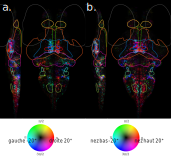
\includegraphics[width=1\textwidth]{./files/tilt_roll.svg.png}
\caption{Cartes de réponses obtenues pour une stimulation de rotation sinusoidale selon l'axe de roulis (a) et de tangage (b). On remarque que la carte est antisymétrique dans le cas du roulis et symétrique dans le cas du tangage.
}
\end{figure}
    
